\documentclass[11pt]{article}
\usepackage{geometry}                
\geometry{letterpaper}                   

\usepackage{graphicx}
\usepackage{float}
\usepackage{algpseudocode}
\usepackage{algorithm}
\usepackage{afterpage}
\usepackage{amssymb}
\usepackage{epstopdf}
\usepackage[framed,numbered,autolinebreaks,useliterate]{mcode}
\usepackage{natbib}
\usepackage{amssymb, amsmath}
\usepackage{microtype}
\usepackage{hyperref}
\usepackage{xcolor}
\hypersetup{
%   %% my addds
	pagebackref=TRUE,
        pdftitle={Network-Based Modeling for the Spread of Scientific Ideas},%
        pdfauthor={M. Berm\'udez, S. Grimm, R. Hosseini},%
        citecolor=blue,%
        linkcolor=blue,%
	hidelinks=TRUE,
	pdfpagemode=UseOutlines,
}


\DeclareGraphicsRule{.tif}{png}{.png}{`convert #1 `dirname #1`/`basename #1 .tif`.png}

\title{Network-Based Modeling for the Spread of Scientific Ideas}
\author{Mayra Berm\'udez, Sarah Grimm, Rzgar Hosseini}
\date{December 14th, 2012} 

\begin{document}



\thispagestyle{empty}

\begin{center}

\includegraphics[width=5cm]{ETHlogo.eps}

\bigskip


\bigskip


\bigskip


\LARGE{ 	Lecture with Computer Exercises:\\ }
\LARGE{ Modelling and Simulating Social Systems with MATLAB\\}

\bigskip

\bigskip

\small{Project Report}\\

\bigskip

\bigskip

\bigskip

\bigskip


\begin{tabular}{|c|}
\hline
\\
\textbf{\LARGE{Network Based Modelling for the Spread of Scientific Ideas}}\\ %center the box with title
%\textbf{\LARGE{...}}\\
\hline
\end{tabular}
\bigskip

\bigskip

\bigskip

\LARGE{Mayra Berm\'udez, Sarah Grimm \& Sayed-Rzgar Hosseini}



\bigskip

\bigskip

\bigskip

\bigskip

\bigskip

\bigskip

\bigskip

\bigskip

Zurich\\

December 14th, 2012\\

\end{center}





\newpage

%%%%%%%%%%%%%%%%%%%%%%%%%%%%%%%%%%%%%%%%%%%%%%%%%

%Agreement for free download

\section*{Agreement for free-download}
\bigskip


\bigskip


\large We hereby agree to make our source code for this project freely available for download from the web pages of the SOMS chair. Furthermore, we assure that all source code is written by ourselves and is not violating any copyright restrictions.


\begin{center}
\vspace{3cm}
Mayra Berm\'udez \hspace{3cm} Sarah Grimm \hspace{2cm} Sayed-Rzgar Hosseini

\end{center}

\newpage



\newpage


%%%%%%%%%%%%%%%%%%%%%%%%%%%%%%%%%%%%%%%



\newpage

\begin{figure}
%[ht]
\begin{center}
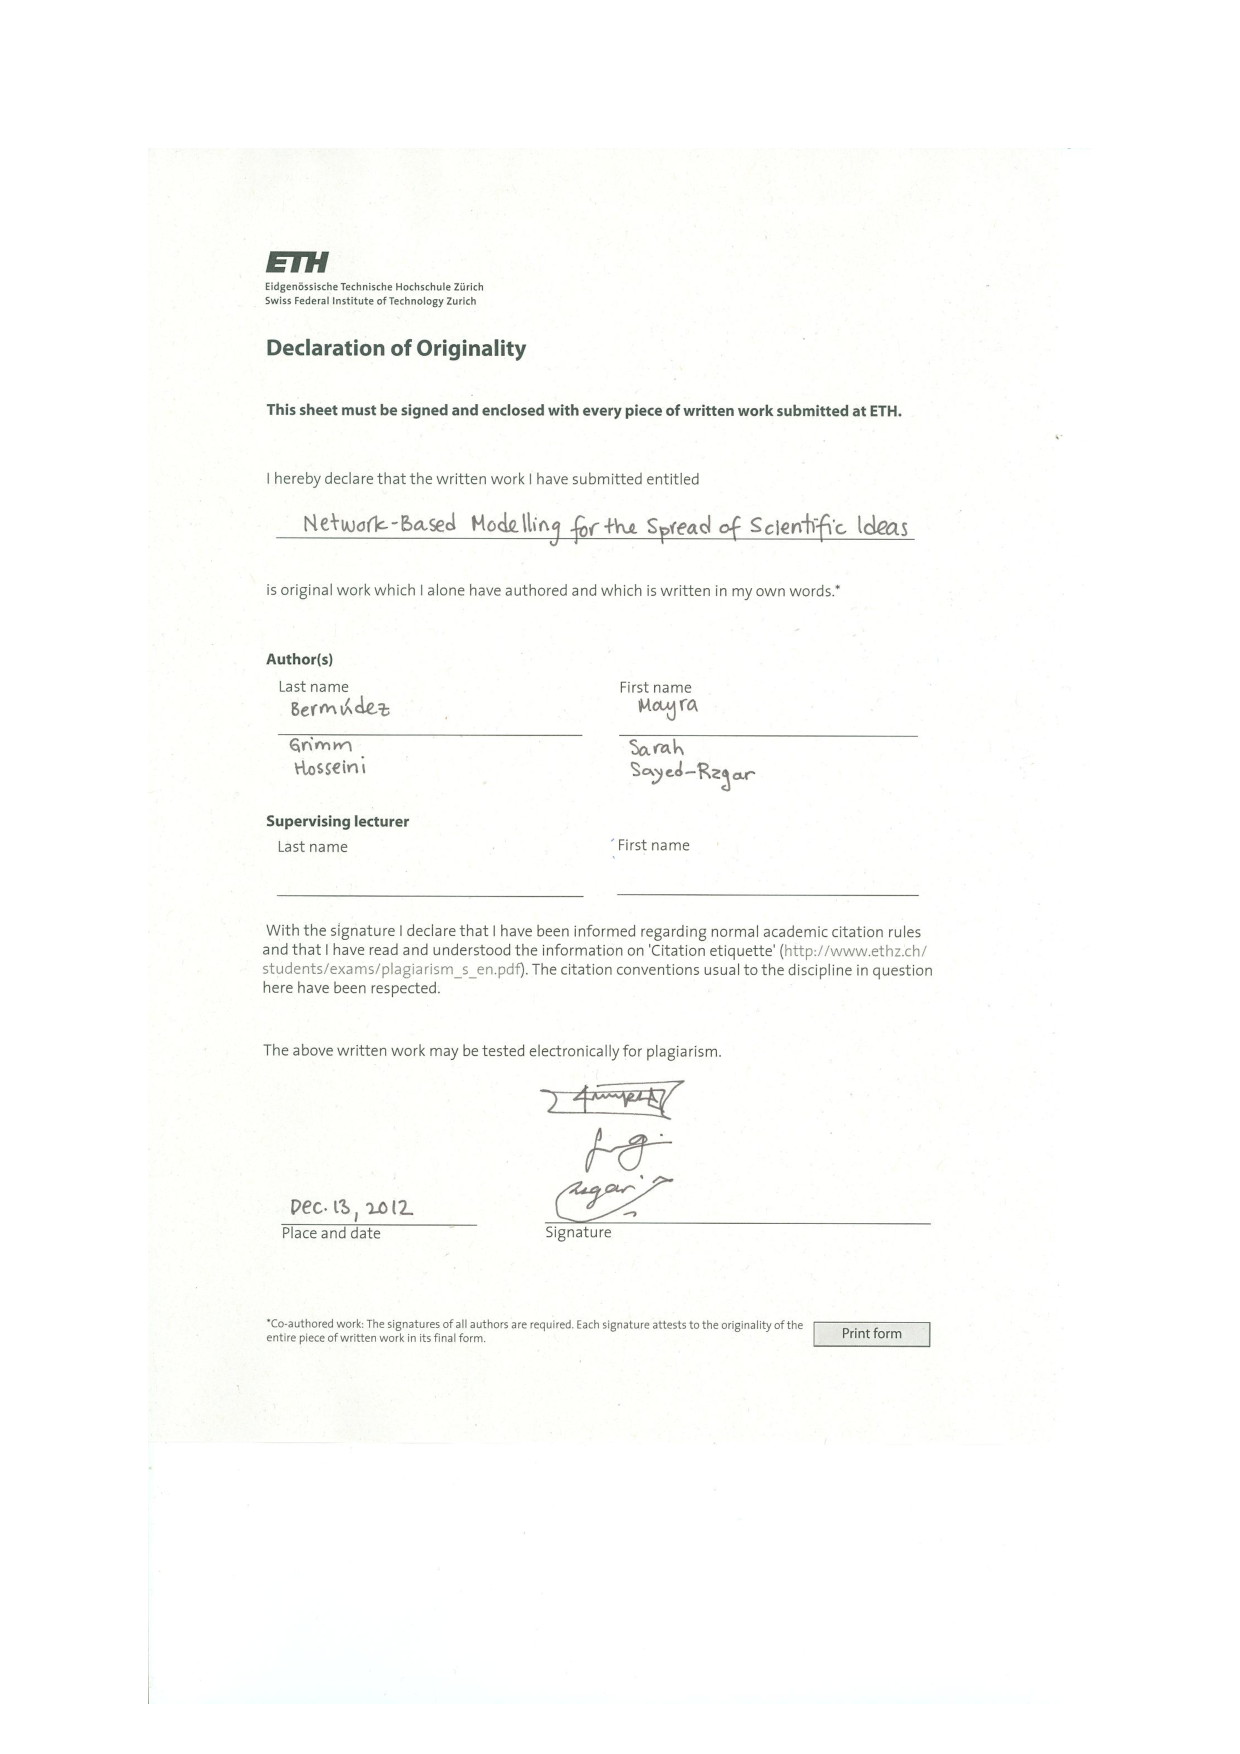
\includegraphics{dec}
\end{center}
\end{figure}
\clearpage
\newpage

\afterpage{\clearpage}


%\clearpage

%\newpage

% IMPORTANT
% you MUST include the ETH declaration of originality here; it is available for download on the course website or at http://www.ethz.ch/faculty/exams/plagiarism/index_EN; it can be printed as pdf and should be filled out in handwriting


%%%%%%%%%% Table of content %%%%%%%%%%%%%%%%%
\newpage
\tableofcontents
\newpage

%%%%%%%%%%%%%%%%%%%%%%%%%%%%%%%%%%%%%%%



\section{Abstract}
%Abstract

%Abstract

Using simulations, we investigated the changes in networks with nodes that held different `scientific ideas' and influenced each other through a complex contagion mechanism. This was divided into two parts: by varying the network structure and observing features of the distribution of ideas in networks, and by varying the starting idea distributions of the nodes and observing features of the network structures. The update step included a rewiring probability, a complex contagion threshold, and a probability of innovation (producing a new idea). We found that both structures and idea distributions influenced each other's features. Values of the update parameter also played a role.
\newpage

\section{Individual contributions}
%Individual Contributions

This report represents a group effort by all members.
\newpage

\section{Introduction and Motivation}
%Introduction and Motivation

We live in a time in which aspects of our lives and of our world become more and more connected with each other. To understand one aspect, we must understand many other aspects, which all together form a large, complex system, or network. Globalization has changed the meaning of `distance' and communication, allowing seemingly unrelated and unconnected individuals to share more than they ever could before. Fields of studies are overlapping with each other, creating new interdisciplinary domains and building a diverse playground for the sharing of ideas. But how do ideas spread? This question is especially interesting with the increase of technology that allows us to record and visualize the networks that connect individuals and ideas, and in particular the ability to `see' how they change. This can lead to insight about why and when ideas spread and into the complexity of the matter. Research has shown that not only does the nature of information or innovation influence the diffusion of it, but also that the structure of a network influences the diffusion dynamics. Here, we try to simulate the spread of scientific ideas in different networks. The model presented is based on two studies: one that investigated critical parameter values for complex contagion \citep{CM2007} and another that investigated critical values of a rewiring parameter \citep{HN2006}.

\subsection{Fundamental Questions}

The main goals of this simulation study are to investigate how network structure influences the distribution of ideas, and how the distribution of ideas influences network structure. For a list of the terminology that will be used throughout the paper, please refer to Table \ref{Tab2}. By varying three parameters - probability of rewiring, rate of innovation, and complex contagion threshold ($\phi$, $\alpha$, and $\delta$ respectively) - and using different network structures and idea distributions, we observed how network structure characteristics changed. Similarly, we observed how the distribution of ideas and the connections between them changed. Below we describe our questions more specifically.

\begin{table}[ht]
\caption{List of terminology} % title of Table
\centering % used for centering table
\begin{tabular}{c c c c } % centered columns (4 columns)
\hline\hline %inserts double horizontal lines
 & Term\\ [0.5ex] % inserts table
%heading
\hline % inserts single horizontal line
Neighborhood index & The fraction of the holders of the same idea\\
\,&  who are neighbor as well averaged over all ideas.\\
\hline
Intra-idea distance& The average distance between \\
&holders of the same idea in the network.\\
\hline
Dominant frequency & The frequency of the dominant idea\\
& in the network at each time steps of the
simulation.\\
\hline
Average dominance time& The average number of time steps \\
&in which the dominant idea keeps its
dominance.\\
\hline
Novelty index& The fraction of newly generated ideas.\\
\hline
Average shortest path & The average number of steps\\
& along the shortest paths for all possible pairs of network nodes.\\
\hline
Clustering coefficient &  A measure of degree to which\\
& nodes in a graph tend to cluster together.\\
\hline
Degree of connectivity &  The number of edges incident to the vertex.\\
\hline
Connected component & A subgraph in which any two vertices are\\
 &connected to each other by paths, and which is connected to no\\
  &additional vertices in the supergraph.\\
\hline
Diameter of network& The longest of all the calculated shortest paths\\
& in a network.\\
\\ [1ex] % [1ex] adds vertical space
\hline %inserts single line
\end{tabular}
\label{Tab2} % is used to refer this table in the text
\end{table}




\subsubsection{Effects of Network Structure on Idea Distribution}

Given a starting network and a random idea distribution, how do different network structures affect the distance between nodes that have the same idea (intra-idea distance)? How do they affect the neighbourhood index? How do they change the emergence of dominant ideas and their time of dominance? How do their effects depend on the values of $\phi$, $\alpha$ and $\delta$?


More rigid network structures (those with less `randomness', such as the caveman and the small world networks) may make it more difficult for `like-minded' nodes (that is, nodes with the same idea) to connect and may thus have smaller neighbourhood indexes and larger intra-idea distances than the more random network structures (such as the random and scale-free networks). Their effects may be more sensitive to the values of $\phi$ (because this affects how likely it is for their structure to change) and to values of $\delta$ because being restricted to a more closed group of nodes makes it difficult to reach a threshold necessary to become similar to surrounding nodes. Values of $\alpha$ may decrease the neighbourhood indexes by creating larger diversity among neighbouring nodes.

If more rigid network structures do make it more difficult for like-minded nodes to connect, then it would be more difficult for a dominant idea to emerge in these networks. These effects may be smaller for larger values of $\phi$ since these values would allow for the structure to change more. For larger values of $\phi$ therefore one could expect that the effects of the network structures on the characteristics of the idea distribution are more similar since allowing to change the structure removes their initial influence.


\subsubsection{Effects of Idea Distribution on Network Structure}

Given a starting idea distribution and a caveman network structure, how do different idea distributions affect the average path length and diameter of the network? Do they change the number of connected components in the network? Do clusters form differently, and how does the clustering coefficient change? What does the distribution of node degree looks like? How do these effects depend on the values of $\phi$, $\alpha$, and $\delta$?


If the starting idea distribution is parallel to the caveman network structure (see Table \ref{Tab2} for definitions), then like-minded nodes will already be connected and thus rewiring will probably not change much of the average path length, nor will it change the diameter. Similarly, the clustering coefficient will remain high just like the starting value. The distribution of the node degree will also not change (nodes will have one of two values for their degree). In other words, if the idea distribution is parallel to the network structure, the structure will not change much. Changing $\phi$ and $\delta$ will not change these effects, and perhaps increasing $\alpha$ will decrease the clustering coefficient and will increase the number of connected components because nodes will disconnect from nodes with novel ideas and will rewire to nodes with the same idea.

If the starting idea distribution is random, then the network's caves will disintegrate as nodes will rewire with other nodes outside of their caves. This will change the degree distribution by increasing its variance (nodes will have a variety of different degree values). Depending on the value of $\delta$ this disintegration may be reduced because nodes have a higher chance of forming dominant ideas within caves. Similarly, increasing $\phi$ will increase the disintegration of caves. Thus for this idea distribution the parameter values may play a larger role.

If the starting idea distribution is anti-parallel, nodes within each cave will initially be connected with nodes that do not hold the same idea as them. Therefore the threshold $\delta$ will not be met in order for nodes to change their ideas, and they will rewire with other nodes outside of their cave. The clustering coefficient and the number of connected components will likely decrease, and the diameter and the average path length will decrease as well since the structure will change significantly. The degree distribution will increase in variance. Increasing $\phi$ and $\alpha$ and decreasing $\delta$ will probably increase the magnitude of these effects. Thus, having an anti-parallel idea distribution will probably display the most changes in the characterstics of the network structure that are in question.




\newpage

\section{Description of the Model}
%Description of the Model


The model used here is based on a study by \citet*{HN2006}.  Each simulation begins with a specified network structure as well as a distribution of the `idea' (or state) of the nodes. At each time step a node either changes its idea to that of one of its neighbors' ideas if its frequency surpasses a defined threshold, rewires to connect with a node that has the same idea, or generates a novel idea (this is the innovation parameter). 


Given the network structure and node states, three parameters are introduced: $\phi$ (probability of rewiring), $\alpha$ (probability of innovation), and $\delta$ (node threshold). As in \citet*{HN2006}, $\phi$ is a value from zero to one, and is the probability that one of the edges of a chosen node \emph{i} \textit{i} will be changed to connect to another node j that i is unconnected with. We decided to add one more criterion to this definition: node j is a node that has the same idea as node i. This encourages the simulations to reflect a common tendency of individuals to seek out others who think like them.


At each time step a node may `come up with a new idea' with a probability of $\alpha$. This value is small to reflect that novel ideas are not frequently observed.


We introduced a node threshold $\delta$ to the general model in order to investigate the behaviour of complex contagion as opposed to simple contagion. This was motivated by a study by \citet*{CM2007}. Simple contagion is well suited for modeling the spread of diseases since they may often be passed on by a single contact with an uninfected individual. However, as our intuition may suggest, and as studies have shown, the spread of other kinds of innovations require several exposures before they are adopted by individuals; these dynamics of diffusion refer to complex contagion.


\subsection{Networks}

For the purposes of our simulations, we used four network structures. These structures can be characterized by properties such as average shortest path lengths, clustering coefficients, and the degree of connectivity. For a brief definition of these properties (which will be used in the results section), please see Table ***** Below are short descriptions of each network structure.

\subsubsection{Random Graph}

The second variant of the Erd\H{o}s-R\'enyi random graph model \citep*{ER1960} as mentioned in \citet{Wiki}, and implemented by \citet*{BS2011}.
Random graphs have a short average path length. The graph is defined by the total number of nodes, and by the probability of any two nodes to be connected. They typically have a small clustering coefficient.

\subsubsection{Caveman Graph}

As defined by \citet*{W2003}.
The caveman structure is defined as having k isolated and fully connected `cliques' where one link is changed to connect one clique to another, rendering all cliques to be connected. Thus, relative to random graphs, they have a high clustering coefficient and a large average shortest path length.

\subsubsection{Small World Graph}

Defined by \citet*{WS1998}, and implemented by \citet*{BS2011}.
Small-world networks have characteristics that lie in between random graphs and highly clustered graphs (such as caveman graphs): they have a high clustering coefficient similar to the latter, but also have a small average shortest path similar to the former. Many real-world networks have been observed to have a small-world structure, and thus we included it in our simulations.

\subsubsection{Scale-Free Graph}

Defined by \citet*{BA1999}, and implemented by \citet*{BS2011}.
Scale-free network structures are often found where new nodes are constantly being added, and they are connected to already well-connected nodes. Such a structure displays a scale-free power-law distribution of the degree (connectivity) of nodes. Thus, there are few nodes that are highly connected, and more nodes that are moderately or mildly connected. Compared to random graphs, they have a smaller average shortest path.
In order to compare between different graph structures, the parameters were chosen such that the mean degree of the graphs were similar (approximately 30). For further details about parameter values, see Table ****

\subsection{Ideas}


After choosing a starting structure for our model, we then chose a distribution for the starting ideas (states) of nodes. The maximum number of different starting ideas is 100. Each node is randomly assigned one of these ideas. For the caveman structure, however, there were two other options: to either distribute the starting ideas `parallel' to the structure, i.e. such that all nodes in a cave shared the same idea, or `antiparallel' such that all nodes in a cave had a different idea. Why. As previously mentioned, each node had a small probability of adopting a novel idea from a virtually unlimited number of new ideas.
\newpage

\section{Implementation}
Our simulation comprises mainly two parts, the phase 1 corresponding to the study  of the effect of network structure on to the opinion distribution and phase 2 where we study how the distribution of the ideas affect the topology of the network. These two phases "runs" in the same MATLAB file called \textbf{mainscript.m}. In both phases the structure of the program is pretty much the same, the difference lies in that in the first one the simulation is done in one of four possible network models: random structure, caveman structure, free scale structure and small world. In the second phase we always work with the same structure: caveman. 
in both phases the structure is formed by 3 steps

\textbf{Step 1:} Structure network is chosen and we generate the adjacency matrix corresponding to that structure.\\
\textbf{Step 2:} The rewiring processes is done using the chosen structure network.\\
\textbf{Step 3:} At this step a eerie of functions are called to getting the results.

\subsection{Step 1: Generating structure networks}

For the first phase one of the functions $step1_scalefree$, $step1_caveman$, $step1_randomgraph$ and $step1_smallworld$ is called, depending in our choice. Each function is found in the MATLAB files \textbf{$step1_scalefree.m$, $step1_caveman.m$, $step1_randomgraph.m$ and $step1_smallworld.m$ } correspondingly.  Each of one functions generates de adjacency matrix corresponding to the network structure. 

For the second phase we just generate the adjacency matrix for the caveman structure network.


\subsection{Step 2: Rewiring}

This step is the same for both phases.

Rewiring simulation is implemented in the file \textbf{step2.m} and done by function \textbf{step2} which requires the next parameters:
\begin{itemize}

\item $t_end$: number of iterations
 \item $phi$:  network reorganization rate
 \item $alpha$: innovation rate
\item $ mat$: initial connectivity matrix
\item  $vec$: initial idea vector
\item $p$: initial number of opinions
 \end{itemize}
 
 And has as outputs:
 \begin{itemize}
 \item $mat$: connectivity matrix after simulation
\item $vec$: idea vector after simulation
\item $dominant\_freq$: the vector holding the frequency of dominant idea
 \item $most\_freq$: the vector holding the index of dominating idea in each time
\end{itemize}

This function follows the next algorithm:

\begin{algorithm}                      % enter the algorithm environment
\caption{Rewiring}          % give the algorithm a caption
\label{alg1}                           % and a label for \ref{} commands later in the document
\begin{algorithmic}                    % enter the algorithmic environment
   % \Require $n \geq 0 \vee x \neq 0$
    %\Ensure $y = x^n$
    %\State $y \Leftarrow 1$
    \For {each of the $t_{end}$ iterations}
    	\State choose a person $x1$ in the network at random
	\State generate a random number $a1$
    \If{$a1 < \phi$} \Comment{ With probability $\phi$ we reorginize the network}
        \State eliminate the connection between $x1$ and one of his neighbourghs with different idea
        \State select at random among the persons with the same idea than $x1$ and that are not already neighbourgs of $x1$ and create a connection between them
    \Else change the idea of $x1$ to one of the ideas of his neighbors which meet the threshold 
            \EndIf
    \State choose a person $y$ in the random to come up with a nobel idea
    \State generate a random number $a2$
    \If $a2<\alpha$ \Comment {With probability $\alpha $ $ y$ comes up with a new idea}
     \EndIf
   \EndFor
\end{algorithmic}
\end{algorithm}

\subsection{Step 3: Getting results}

In the phase 1 we want to observe the influence of a certain network structure  on the distribution of ideas after the rewiring process (step 2). For this is necessary to search for parameters that reflects the final distribution of ideas. In this study we observe the following parameters:

\begin{itemize}
\item $n_index$ which is the average neighbour index of the network
\item average $intra_distance$ between agentsholding the same idea
\item $average_time$ which is the average of the dominance time for different dominance periods
\end{itemize}

All this parameters are calculated in \textbf{step3a.m, step3b.m and step 3d.m} which are called in $main_scrpipt.m.$

In phase 2 we want to find out how the distribution of ideas change the network structure, for this reason we just see at caveman structure, and after step 2 we want to see how the initial structure was modified by the rewiring process. To see that we look for the next parameters

\begin{itemize}
\item the clustering coefficient of a network
\item  degree vector (dgr) and its corresponding
\item the average path length for the graph
\item outputs the diameter of the graph 'mat'

\end{itemize}








      
\newpage

\section{Simulation Results and Discussion}
%Results and Discussion
\newpage

\section{Summary and Outlook}
%Summary and Outlook

To conclude our simulation study, our results support the general idea that network structure and qualities of the ideas held in them may mutually influence each other. The more rigid the structure of a network was, the more likely that the intra-idea distance and neighbourhood index of the network was larger. These two features varied more with the innovation rate $\alpha$ for less structured networks, and varied more with the complex contagion threhold $\delta$ for the most rigid structure - the caveman network. The average dominance time seemed to vary more with parameter values ($\phi$, $\delta$, and $\alpha$) than with the network structures, whereas the frequency of dominance of ideas did not decrease on average in the long run with any network structure.

A network in which the pattern of ideas held by the nodes are `in accord' within the clusters of the caveman network maintained more of the structure features of a caveman network. These values varied with values of rewiring probabilities $\phi$ and complex contagion threholds $\delta$. Networks with a random pattern of ideas or with a pattern with more `disaccord' within the clusters resulted in a structure that began to resemble a random graph more than a caveman network. These networks' values varied more with the parameter $\phi$ of rewiring. Nodes given the chance to rewire with nodes that share the same idea had more opportunity to do so in the random and `disaccord' idea patterns than in the pattern which already had much accord.

Thus, in addition to the structure of networks and the pattern of ideas in them, complex contagion thresholds, innovation rates, and the probability of creating new connections (while reflecting `preferences' of being connected with like-minded others) tend to influence features of the network. Several extensions to the proposed model could be investigated to better understand the relationships between network structure and idea distribution.

\paragraph{Rewiring criteria}
Future simulations may compare the emerging features of idea distributions not just between network structures, but also between different rewiring criteria. It is not clear how much of the features of the idea distribution in this simulation study was a result of the network structure or of the `preference' that nodes had in rewiring to like-minded nodes. Therefore, these results could be compared to (1) random rewiring or, to allow structure to play a larger role, (2) to allow random rewiring to nodes that are at most a distance of three nodes away. This is somewhat more realistic since most people connect with individuals who are somewhat in their vicinity through mutual connections. 

\paragraph{Complex contagion and innovation}
Considering complex contagion, novel ideas in our model were at a disadvantage for spreading in the network. Allowing novel ideas to have a larger influence weight may be one way to grant the ability of them to spread to other nodes. Alternatively, the complex contagion threshold for novel ideas may be lowered.

\paragraph{Random idea adoption}
Future simulations may investigate the effects of network structure on idea distributions by comparing to a `benchmark' model. This model would update the ideas of nodes at random, and thus the effects of connections may be better observed within network structures and then compared between network structures.




\newpage


\bibliographystyle{plain}

\bibliography{Refs}
\newpage

\appendix
\textbf{Main Step}

\input{MainStep}

\textbf{Random graph}

\textbf{Scale free}

\textbf{Small world}

\textbf{Caveman}

\textbf{Step 1 Caveman}

\textbf{Step 1 Random graph}

\textbf{Step 1 Small world}

\textbf{Step 2}

\textbf{Step 3a}

\textbf{Step 3b}

\textbf{Step 3e}

\textbf{Step 4a}

\textbf{Step 4b}

\textbf{Step 4d}

\textbf{Step 4e}






\end{document}  